\documentclass[a4paper,12pt]{article} % добавить leqno в [] для нумерации слева
\usepackage[a4paper,top=1.3cm,bottom=2cm,left=1.5cm,right=1.5cm,marginparwidth=0.75cm]{geometry}
%%% Работа с русским языком
\usepackage{cmap}					% поиск в PDF
\usepackage{mathtext} 				% русские буквы в фомулах
\usepackage[T2A]{fontenc}			% кодировка
\usepackage[utf8]{inputenc}			% кодировка исходного текста
\usepackage[english,russian]{babel}	% локализация и переносы
\usepackage{multirow}

\usepackage{graphicx}

\usepackage{wrapfig}
\usepackage{tabularx}

\usepackage{hyperref}
\usepackage[rgb]{xcolor}
\hypersetup{
colorlinks=true,urlcolor=blue
}

%%% Дополнительная работа с математикой
\usepackage{amsmath,amsfonts,amssymb,amsthm,mathtools} % AMS
\usepackage{icomma} % "Умная" запятая: $0,2$ --- число, $0, 2$ --- перечисление

%% Номера формул
\mathtoolsset{showonlyrefs=true} % Показывать номера только у тех формул, на которые есть \eqref{} в тексте.

%% Шрифты
\usepackage{euscript}	 % Шрифт Евклид
\usepackage{mathrsfs} % Красивый матшрифт

%% Свои команды
\DeclareMathOperator{\sgn}{\mathop{sgn}}

%% Перенос знаков в формулах (по Львовскому)
\newcommand*{\hm}[1]{#1\nobreak\discretionary{}
{\hbox{$\mathsurround=0pt #1$}}{}}

%% Графики
\usepackage{tikz}
\usepackage{pgfplots}
\pgfplotsset{compat=1.9}

\date{\today}

\begin{document}

\begin{titlepage}
	\begin{center}
		{\large МОСКОВСКИЙ ФИЗИКО-ТЕХНИЧЕСКИЙ ИНСТИТУТ (НАЦИОНАЛЬНЫЙ ИССЛЕДОВАТЕЛЬСКИЙ УНИВЕРСИТЕТ)}
	\end{center}
	\begin{center}
		{\large Физтех-школа аэрокосмических технологий}
	\end{center}
	
	
	\vspace{4.5cm}
	{\huge
		\begin{center}
			{\bf Отчёт о выполнении лабораторной работы 2.1.4}\\
			Определение теплоёмкости твёрдых тел
		\end{center}
	}
	\vspace{1cm}
	\begin{center}
		{\large Соболевский Федор Александрович \\
			\vspace{0.2cm}
			Б03-109}
	\end{center}
	\vspace{8cm}
	\begin{center}
		Март 2022
	\end{center}
\end{titlepage}

\section{Аннотация}

В данной работе изучена теплоёмкость твёрдых тел и методы её определения. Исследована температурная зависимость электрического сопротивления для определение изменения температуры исследуемых образцов. Для учёта теплопотерь зависимость $\Delta Q/ \Delta T$ экстраполирована к нулевым потерям тепла.

\section{Теоретические сведения}

\subsection{Методика определения теплоёмкости}

Теплоёмкость системы определяется отношением

\begin{equation}
    C = \frac{\Delta Q}{\Delta T}.
    \label{capacityDef}
\end{equation}

При измерении количества тепла, поглощаемого телом в калориметре постоянной мощности нагрева, необходимо учитывать потери тепла, обусловленные теплопроводность стенок прибора. В этом случае количество теплоты, поглощаемое телом за время $\Delta t$, определяется как

\begin{equation}
    \Delta Q = P\Delta t - \lambda(T - T_0)\Delta t,
    \label{heat}
\end{equation}

где $P$ - мощность нагревателя, $\lambda$ - коэффициент теплоотдачи стенок калориметра, $T$ - температура тела, $T_0$ - температура окружающей среды (воздуха в лаборатории). Из уравнений \eqref{capacityDef} и \eqref{heat} следует основное расчётное уравнение

\begin{equation}
    C = \frac{P - \lambda(T - T_0)}{\Delta T / \Delta t}.
    \label{main}
\end{equation}

Мощность теплопотерь прямо пропорциональна разности температур тела и окружающего воздуха и при равенстве данных температур стремится к нулю. Для измерения значения $f(T) = \Delta T / \Delta t$ в точке $T = T_0$ следует построить в достаточно широком диапазоне температур график $f(T)$ и экстраполировать его к данной точке. Получая полученное значение $(\Delta T / \Delta t)_{T_0}$ в формулу \eqref{main}, получим

\begin{equation}
    C = \frac{P}{(\Delta T / \Delta t)_{T_0}}.
\end{equation}

Температуру в калориметре можно измерить, зная зависимость электрического сопротивления от температуры: 

\begin{equation}
    R(\Delta T) = R_{273}(1 + \alpha \Delta T),
    \label{resistance}
\end{equation}

где $R_{273}$ - сопротивление при $T = 273$ К, $\alpha$ - известный температурный коэффициент сопротивления, $\Delta T$ - отличие температуры от 0 $^\text{o}$C. Дифференцируя \eqref{resistance} по времени, получим 

\begin{equation}
    \frac{dR}{dt} = R_{273}\alpha\frac{dT}{dt}.
    \label{timeDif}
\end{equation}

Выражая $R_{273}$ из \eqref{resistance} через сопротивление $R_0$ и разность температур $\Delta T_0$ при комнатной температуре

\begin{equation}
    R_{273} = \frac{R_0}{1 + \alpha \Delta T_0},
    \label{res0}
\end{equation}

получим из \eqref{timeDif} и \eqref{res0}

\begin{equation}
    C = \frac{P\alpha R_0}{(\frac{dR}{dt})_{T_0}(1 + \alpha \Delta T_0)}.
    \label{final}
\end{equation}

\subsection{Экспериментальная установка}

\begin{figure}
    \centering
    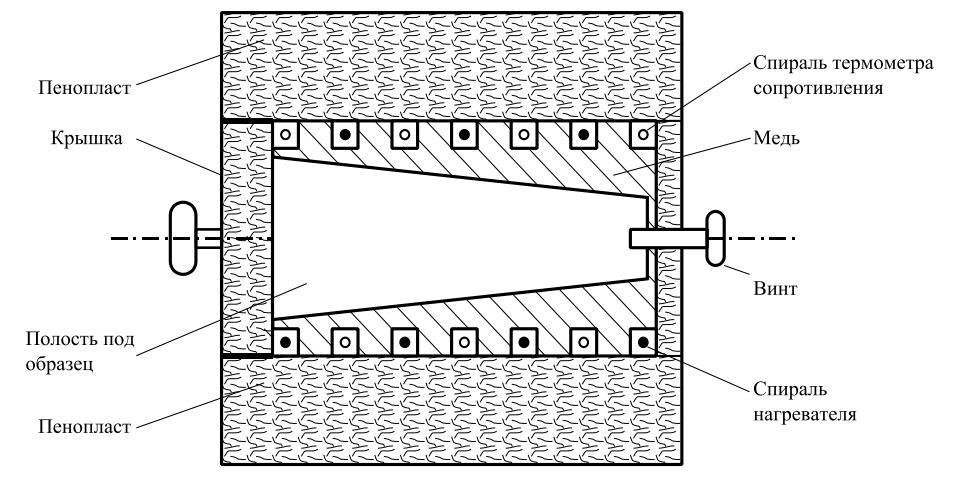
\includegraphics[width = 0.6\textwidth]{setup.PNG}
    \caption{Схема устройства калориметра}
    \label{fig:setup}
\end{figure}

\begin{figure}
    \centering
    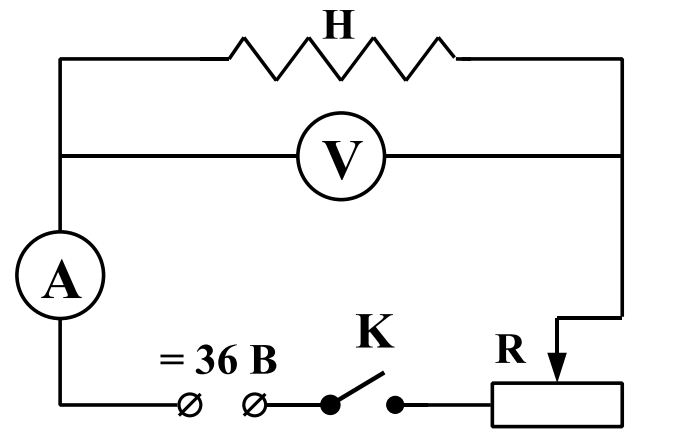
\includegraphics[width = 0.45\textwidth]{circuit.PNG}
    \caption{Схема включения нагревателя}
    \label{fig:circuit}
\end{figure}

Установка состоит из калориметра с пенопластовой изоляцией, помещенного в ящике из многослойной клееной фанеры (см. рис. \ref{fig:setup}). Внутренние стенки калориметра выполнены из материала с высокой теплопроводностью. Надежность теплового контакта между телом и стенками обеспечивается их формой: они имеют вид усеченных конусов и плотно прилегают друг к другу. В стенку калориметра вмонтированы электронагреватель и термометр сопротивления. Схема включения нагревателя изображена на рис. \ref{fig:circuit}. Система реостатов позволяет установить нужную силу тока в цепи нагревателя. По амперметру и вольтметру определяется мощность, выделяемая током в нагревателе. Величина сопротивления термометра измеряется мостом постоянного тока.

\section{Оборудование и инструментальные погрешности}

\textbf{В работе использовались:} калориметр с нагревателем и термометром сопротивления, амперметр, вольтметр, мост постоянного тока, источник питания 36 В, секундомер, термометр.

\textbf{Инструментальные погрешности:}

\begin{itemize}
    \item \textbf{Мост постоянного тока:} $\Delta_R = 0,001$ Ом;
    \item \textbf{Секундомер:} $\Delta_t = 0,01$ с;
    \item \textbf{Термометр:} $\Delta_T = 0,05$ К.
\end{itemize}

\section{Результаты измерений и обработка экспериментальных данных}

\subsection{Подготовка к проведению опыта}

В опытах использовались три тела: цилиндры из железа, алюминия и латуни. Перед проведением опыта были установлены следующие параметры экспериментальной установки и исследуемых тел:

\begin{itemize}
    \item Температурный коэффициент сопротивления меди: $\alpha = 4,28 \cdot 10^{-3}$ К$^{-1}$;
    \item Комнатная температура: $\Delta T_0 = 21,8$ К;
    \item Начальное сопротивление термометра: $R_0 = 18,087$ Ом;
    \item Мощность нагревателя: $P = IV = 0,3$ А $\cdot 36$ В $= 10,8$ Вт;
    \item Масса железного конуса: $m_1 = (813,2 \pm 0,1)$ г;
    \item Масса алюминиевого конуса: $m_2 = (294,2 \pm 0,1)$ г;
    \item Масса латунного конуса: $m_3 = (868,7 \pm 0,1)$ г.
\end{itemize}

\subsection{Определение зависимости сопротивления от времени}

Для определения зависимости сопротивления от времени для пустого калориметра и для калориметра с каждым из трёх исследуемых образцов было измерено время установления четырнадцати значений сопротивления с равным интервалом $\Delta R = 0,05$ Ом. Полученные значения изображены в таблице \ref{tab:resistances}. Графики зависимости сопротивления от времени показаны на рис. \ref{graph1}.

\begin{table}[]
    \centering
    \begin{tabular}{|c|c|c|c|c|c|c|c|}\hline
        \multicolumn{8}{|c|}{Пустой калориметр}\\ \hline
        $R$, Ом & 18,137 & 18,187 & 18,237 & 18,287 & 18,337 & 18,387 & 18,437 \\ \hline
        $\Delta t$, с & 51,64 & 53,20 & 54,62 & 55,64 & 57,04 & 60,4 & 58,78 \\ \hline
        $t$, с & 51,64 & 104,84 & 159,46 & 215,10 & 272,14 & 332,54 & 391,32 \\ \hline 
        $R$, Ом & 18,487 & 18,537 & 18,587 & 18,637 & 18,687 & 18,737 & 18,787 \\ \hline
        $\Delta t$, с & 61,76 & 64,78 & 65,15 & 67,00 & 68,21 & 73,12 & 73,07 \\ \hline
        $t$, с & 453,08 & 517,86 & 583,01 & 650,01 & 718,22 & 791,34 & 864,41 \\ \hline 
        \multicolumn{8}{|c|}{Калориметр с железным цилиндром}\\ \hline
        $R$, Ом & 18,137 & 18,187 & 18,237 & 18,287 & 18,337 & 18,387 & 18,437 \\ \hline
        $\Delta t$, с & 75,03 & 76,41 & 78,80 & 80,53 & 83,32 & 86,14 & 87,9 \\ \hline
        $t$, с & 75,03 & 151,44 & 230,24 & 310,77 & 394,09 & 480,23 & 568,13 \\ \hline
        $R$, Ом & 18,487 & 18,537 & 18,587 & 18,637 & 18,687 & 18,737 & 18,787 \\ \hline
        $\Delta t$, с & 89,63 & 93,67 & 93,70 & 97,37 & 102,13 & 101,68 & 103,13 \\ \hline
        $t$, с & 657,76 & 751,43 & 845,13 & 942,50 & 1044,63 & 1146,31 & 1249,44 \\ \hline
        \multicolumn{8}{|c|}{Калориметр с алюминиевым цилиндром}\\ \hline
        $R$, Ом & 18,137 & 18,187 & 18,237 & 18,287 & 18,337 & 18,387 & 18,437 \\ \hline
        $\Delta t$, с & 61,42 & 64,28 & 67,34 & 68,06 & 72,95 & 72,37 & 74,55 \\ \hline
        $t$, с & 61,41 & 125,70 & 193,04 & 261,10 & 334,05 & 406,42 & 480,97 \\ \hline
        $R$, Ом & 18,487 & 18,537 & 18,587 & 18,637 & 18,687 & 18,737 & 18,787 \\ \hline
        $\Delta t$, с & 76,96 & 80,07 & 82,58 & 82,51 & 85,07 & 88,34 & 91,11 \\ \hline
        $t$, с & 557,93 & 638,00 & 720,58 & 803,09 & 888,16 & 976,5 & 1067,61 \\ \hline
        \multicolumn{8}{|c|}{Калориметр с латунным цилиндром}\\ \hline
        $R$, Ом & 18,137 & 18,187 & 18,237 & 18,287 & 18,337 & 18,387 & 18,437\\ \hline
        $\Delta t$, с & 64,23 & 66,68 & 72,15 & 74,83 & 76,73 & 79,84 & 82,35\\ \hline
        $t$, с & 64,23 & 130,91 & 203,06 & 277,89 & 354,62 & 434,46 & 516,81\\ \hline
        $R$, Ом & 18,487 & 18,537 & 18,587 & 18,637 & 18,687 & 18,737 & 18,787\\ \hline
        $\Delta t$, с & 81,34 & 88,04 & 84,32 & 90,27 & 93,27 & 96,39 & 96,42\\ \hline
        $t$, с & 598,15 & 686,19 & 770,51 & 860,78 & 954,05 & 1050,44 & 1146,86\\ \hline
        \end{tabular}
    \caption{Изменение сопротивления термометра со временем}
    \label{tab:resistances}
\end{table}

\begin{figure}
\centering
\resizebox {0.7\textwidth} {!} {
\begin{tikzpicture}
\begin{axis}[ xlabel = {$t$, с}, ylabel = {$R$, Ом}, xmin = 0, xmax = 1250, ymin = 18.087, ymax = 18.8, legend style={legend style={at={(axis cs:1250, 18.087)},anchor=south east}}]

\addplot[color=black, mark=square] coordinates{
(0, 18.087)
(51.64, 18.137)
(104.84, 18.187)
(159.46, 18.237)
(215.1, 18.287)
(272.14, 18.337)
(332.54, 18.387)
(391.32, 18.437)
(453.08, 18.487)
(517.86, 18.537)
(583.01, 18.587)
(650.01, 18.637)
(718.22, 18.687)
(791.34, 18.737)
(864.41, 18.787)};
\addplot[color=blue, mark=o] coordinates{
(0, 18.087)
(75.03, 18.137)
(151.44, 18.187)
(230.24, 18.237)
(310.77, 18.287)
(394.09, 18.337)
(480.23, 18.387)
(568.13, 18.437)
(657.76, 18.487)
(751.43, 18.537)
(845.13, 18.587)
(942.5, 18.637)
(1044.63, 18.687)
(1146.31, 18.737)
(1249.44, 18.787)};
\addplot[color=purple, mark=triangle] coordinates{
(0, 18.087)
(61.42, 18.137)
(125.5, 18.187)
(193.04, 18.237)
(261.1, 18.287)
(334.05, 18.337)
(406.42, 18.387)
(480.97, 18.437)
(557.93, 18.487)
(638, 18.537)
(720.58, 18.587)
(803.09, 18.637)
(888.16, 18.687)
(976.5, 18.737)
(1067.61, 18.787)};
\addplot[color=red, mark=*] coordinates{
(0, 18.087)
(64.23, 18.137)
(130.91, 18.187)
(203.06, 18.237)
(277.89, 18.287)
(354.62, 18.337)
(434.46, 18.387)
(516.81, 18.437)
(598.15, 18.487)
(686.19, 18.537)
(770.51, 18.587)
(860.78, 18.637)
(954.05, 18.687)
(1050.44, 18.737)
(1146.86, 18.787)};

\legend{Пустой, Железный, Алюминиевый, Латунный}

\end{axis}
\end{tikzpicture}
}
\caption{Зависимость сопротивления от времени нагрева}
\label{graph1}
\end{figure}

Далее приведена зависимость производной сопротивления по времени от времени: для каждого участка времени найдено отношение $\Delta R/\Delta t$. Полученные значения отражены в таблице \ref{tab:difs}. График полученной зависимости изображён на рис. \ref{graph2}.

\begin{table}[]
    \centering
    \begin{tabular}{|c|c|c|c|c|c|c|c|}\hline
        \multicolumn{8}{|c|}{Пустой калориметр}\\ \hline
        $t$, с & 51,64 & 104,84 & 159,46 & 215,10 & 272,14 & 332,54 & 391,32 \\ \hline 
        $\Delta R/\Delta t$, $10^{-4}$ Ом/с & 9,682 & 9,398 & 9,154 & 8,986 & 8,766 & 8,278 & 8,506 \\ \hline 
        $t$, с & 453,08 & 517,86 & 583,01 & 650,01 & 718,22 & 791,34 & 864,41 \\ \hline 
        $\Delta R/\Delta t$, $10^{-4}$ Ом/с & 8,096 & 7,718 & 7,675 & 7,463 & 7,330 & 6,838 & 6,843 \\ \hline
        \multicolumn{8}{|c|}{Калориметр с железным цилиндром}\\ \hline
        $t$, с & 75,03 & 151,44 & 230,24 & 310,77 & 394,09 & 480,23 & 568,13 \\ \hline
        $\Delta R/\Delta t$, $10^{-4}$ Ом/с & 6,664 & 6,544 & 6,345 & 6,209 & 6,001 & 5,805 & 5,688 \\ \hline
        $t$, с & 657,76 & 751,43 & 845,13 & 942,50 & 1044,63 & 1146,31 & 1249,44 \\ \hline
        $\Delta R/\Delta t$, $10^{-4}$ Ом/с & 5,578 & 5,338 & 5,336 & 5,135 & 4,896 & 4,917 & 4,848 \\ \hline 
        \multicolumn{8}{|c|}{Калориметр с алюминиевым цилиндром}\\ \hline
        $t$, с & 61,41 & 125,70 & 193,04 & 261,10 & 334,05 & 406,42 & 480,97 \\ \hline
        $\Delta R/\Delta t$, $10^{-4}$ Ом/с & 8,141 & 7,778 & 7,425 & 7,346 & 6,854 & 6,909 & 6,707 \\ \hline
        $t$, с & 557,93 & 638,00 & 720,58 & 803,09 & 888,16 & 976,5 & 1067,61 \\ \hline
        $\Delta R/\Delta t$, $10^{-4}$ Ом/с & 6,497 & 6,245 & 6,055 & 6,060 & 5,878 & 5,660 & 5,488 \\ \hline
        \multicolumn{8}{|c|}{Калориметр с латунным цилиндром}\\ \hline
        $t$, с & 64,23 & 130,91 & 203,06 & 277,89 & 354,62 & 434,46 & 516,81\\ \hline
        $\Delta R/\Delta t$, $10^{-4}$ Ом/с & 7,785 & 7,499 & 6,930 & 6,682 & 6,516 & 6,263 & 6,072 \\ \hline
        $t$, с & 598,15 & 686,19 & 770,51 & 860,78 & 954,05 & 1050,44 & 1146,86\\ \hline
        $\Delta R/\Delta t$, $10^{-4}$ Ом/с & 6,147 & 5,679 & 5,930 & 5,539 & 5,361 & 5,187 & 5,186 \\ \hline
        \end{tabular}
    \caption{Изменение производной сопротивления термометра по времени}
    \label{tab:difs}
\end{table}

\begin{figure}
\centering
\resizebox {0.7\textwidth} {!} {
\begin{tikzpicture}
\begin{axis}[ xlabel = {$t$, с}, ylabel = {$R$, Ом}, xmin = 0, xmax = 1250, ymin = 4.8, ymax = 9.8, legend style={legend style={at={(axis cs:1250, 9.8)},anchor=north east}}]

\addplot[color=black, mark=square] coordinates{
(51.64, 9.682)
(104.84, 9.398)
(159.46, 9.154)
(215.1, 8.986)
(272.14, 8.766)
(332.54, 8.278)
(391.32, 8.506)
(453.08, 8.096)
(517.86, 7.718)
(583.01, 7.675)
(650.01, 7.463)
(718.22, 7.33)
(791.34, 6.838)
(864.41, 6.843)};
\addplot[color=blue, mark=o] coordinates{
(75.03, 6.664)
(151.44, 6.544)
(230.24, 6.345)
(310.77, 6.209)
(394.09, 6.001)
(480.23, 5.805)
(568.13, 5.688)
(657.76, 5.578)
(751.43, 5.338)
(845.13, 5.336)
(942.5, 5.135)
(1044.63, 4.896)
(1146.31, 4.917)
(1249.44, 4.848)};
\addplot[color=purple, mark=triangle] coordinates{
(61.42, 8.141)
(125.5, 7.778)
(193.04, 7.425)
(261.1, 7.346)
(334.05, 6.854)
(406.42, 6.909)
(480.97, 6.707)
(557.93, 6.497)
(638, 6.245)
(720.58, 6.055)
(803.09, 6.06)
(888.16, 5.878)
(976.5, 5.66)
(1067.61, 5.488)};
\addplot[color=red, mark=*] coordinates{
(64.23, 7.785)
(130.91, 7.499)
(203.06, 6.93)
(277.89, 6.682)
(354.62, 6.516)
(434.46, 6.263)
(516.81, 6.072)
(598.15, 6.147)
(686.19, 5.679)
(770.51, 5.930)
(860.78, 5.539)
(954.05, 5.361)
(1050.44, 5.187)
(1146.86, 5.186)};

\legend{Пустой, Железный, Алюминиевый, Латунный}

\end{axis}
\end{tikzpicture}
}
\caption{Зависимость сопротивления от времени нагрева}
\label{graph2}
\end{figure}

Далее была произведена полиномиальная экстраполяция полученных значений к точке $ t = 0 $ с помощью функции "Полиномиальная линия тренда" в Microsoft Excel. На рис. \ref{fig:trends} изображены полученные линии тренда и их уравнения. Свободный член в уравнениях является значением функции в точке $t = 0$.

\begin{figure}
    \centering
    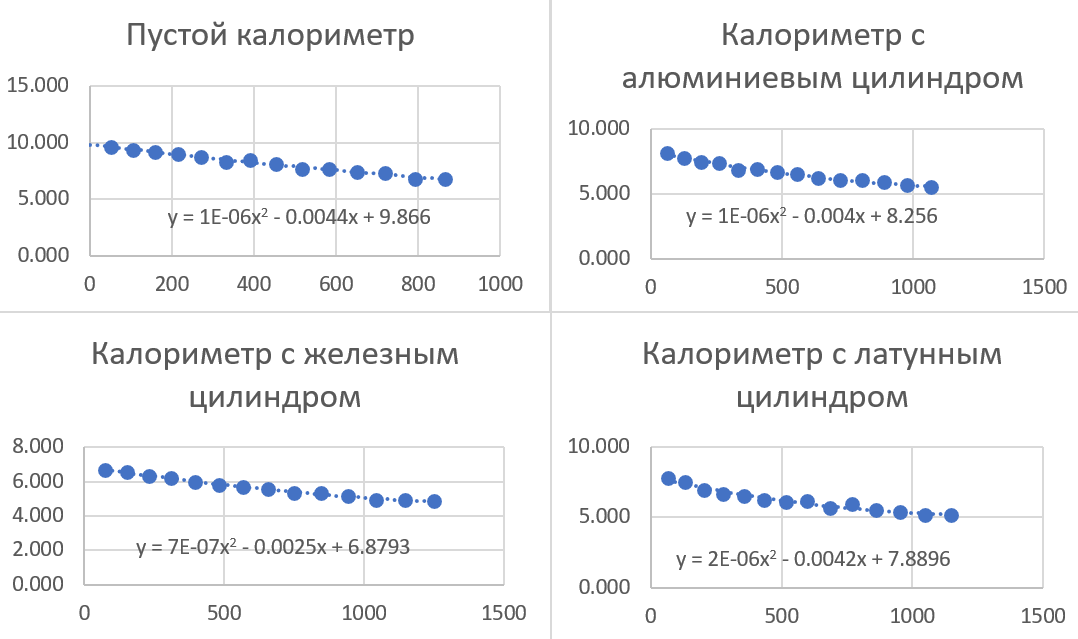
\includegraphics[width = 0.9\textwidth]{trends.PNG}
    \caption{Полиномиальная экстраполяция значений производной сопротивления термометра}
    \label{fig:trends}
\end{figure}

С использованием полученных значений $(dR/dt)_{T_0}$ по формуле \eqref{final} были вычислены значения теплоёмкости системы $C_0$. Значения собственной теплоёмкости цилиндров $C$ определяются как разность теплоёмкости системы $C_0$ и теплоёмкости пустого калориметра. Удельная и молярная теплоёмкости металлов определяются как
\begin{equation}
    c_m = \frac{C}{m},
\end{equation}

\begin{equation}
    c_\nu = \frac{C}{\nu} = \frac{C\mu}{m},
\end{equation}

где $\mu$ - молярная масса металла. Полученные значения коэффициентов наилучших прямых, теплоёмкостей и молярные массы металлов представлены в таблице \ref{tab:results}.

\begin{table}[h]
    \centering
    \begin{tabular}{|c|c|c|c|c|} \hline
    Образец & Пустой & Железный & Алюминиевый & Латунный \\ \hline
    $(dR/dt)_{T_0}$, $10^{-3}$ Ом/с & 9,866 & 6,879 & 8,256 & 7,890 \\ \hline
    $C_0$, Дж/К & 777,23 & 1114,72 & 928,80 & 971,89 \\ \hline
    \multicolumn{2}{|c|}{$C$, Дж/К} & 337,49 & 151,57 & 194,65 \\ \hline
    \multicolumn{2}{|c|}{$c_m$, Дж/кг$\cdot$К} & 415,47 & 515,19 & 224,07 \\ \hline
    \multicolumn{2}{|c|}{$\mu$, кг/моль} & 0,056 & 0,027 & 0,064 \\ \hline
    \multicolumn{2}{|c|}{$c_\nu$, Дж/моль$\cdot$К} & 23,202 & 13,900 & 14,437 \\ \hline
    \end{tabular}
    \caption{Результаты вычисления теплоёмкостей}
    \label{tab:results}
\end{table}

\section{Обсуждение результатов и выводы}

Полученные в ходе эксперимента значения удельных теплоёмкостей исследованных металлов значительно отличаются от табличных: для железа отклонение составило около 10\%, для алюминия - 80\%, для латуни - почти 90\%. Данные отклонения невозможно объяснить одной лишь погрешностью измерений. Рассмотрим возможные причины отклонений.

Наиболее вероятная причина ошибки - неучтённая теплоёмкость воздуха в калориметре. Также калориметр мог быть закрыт недостаточно плотно, что создало возможность его конвективного охлаждения. Также ошибка может быть связана с составом сплавов металлов и образованием на них оксидов. В целом можно сделать, что используемая экспериментальная установка мало применима для измерения теплоёмкостей ввиду своих дефектов.

Данный опыт, однако, показал применимость рассмотренного метода измерения теплоёмкостей, так как по порядку полученные значения не отличаются от табличных. Для проведения точных измерений следует использовать более надёжные установки для минимизации теплопотерь и более точного определения изменения температуры. 

\end{document}
